%***********************************************************
\subsection{MCMC Convergence}\label{sub:bc_mcmc_convergence}
%***********************************************************

% Introductory paragraph
All the calibration schemes explained above were each run for a total of $2'000$ iterations using $1'000$ walkers. 
This will results in a total of $2'000'000$ posterior samples.
However, these initial samples requires further post-processing to remove the initialization bias and incorrect statistical error estimation due to autocorrelation in the samples.
In the following, only the results from the calibration with model bias term are discussed.
The results from other schemes are similar.

% Trace plots
Fig.~\ref{fig:ch5_plot_ens_trace_all_disc_centered} shows the trace plots for each of the $8$ model parameters in the calibration with model bias term.
To avoid over-plotting, shown in the plot are only the trajectories for the last $100$ iterations (out of $1'240$ post-burn-in iterations) and for $400$ walkers (out of $1'000$ walkers). 
As can be seen, the walkers traverse the model parameter space and spend more time during the iterations in the region where it is consistent with the data (thus the region becomes darker in the plots).
Furthermore, it can also be inferred that some parameters are more constrained by the data (e.g., \texttt{gridHT}) than the others (e.g., \texttt{tQuench}).

% Figure MCMC Ensemble Statistics
To check the convergence of the results of an ensemble samplers, it is a common practice to investigate the running statistics of the ensemble (i.e., statistics over all walkers per iteration) instead of the individual walker \cite{Foreman-Mackey2013,Akeret2013}.
The running average and standard deviation for each model parameter are shown in Fig.~\ref{fig:ch5_plot_ens_stat_mcmc}.
The labels for the individual parameters are intentionally left out for the time being.
From the figure, it is clear that after some initial transient (i.e., the burn-in period), the running statistics converge.
Note also that the number the length of the burn-in period for an ensemble sampler tends to be large in proportion to the total number of iterations.
\begin{figure}[!bth]
    \centering
    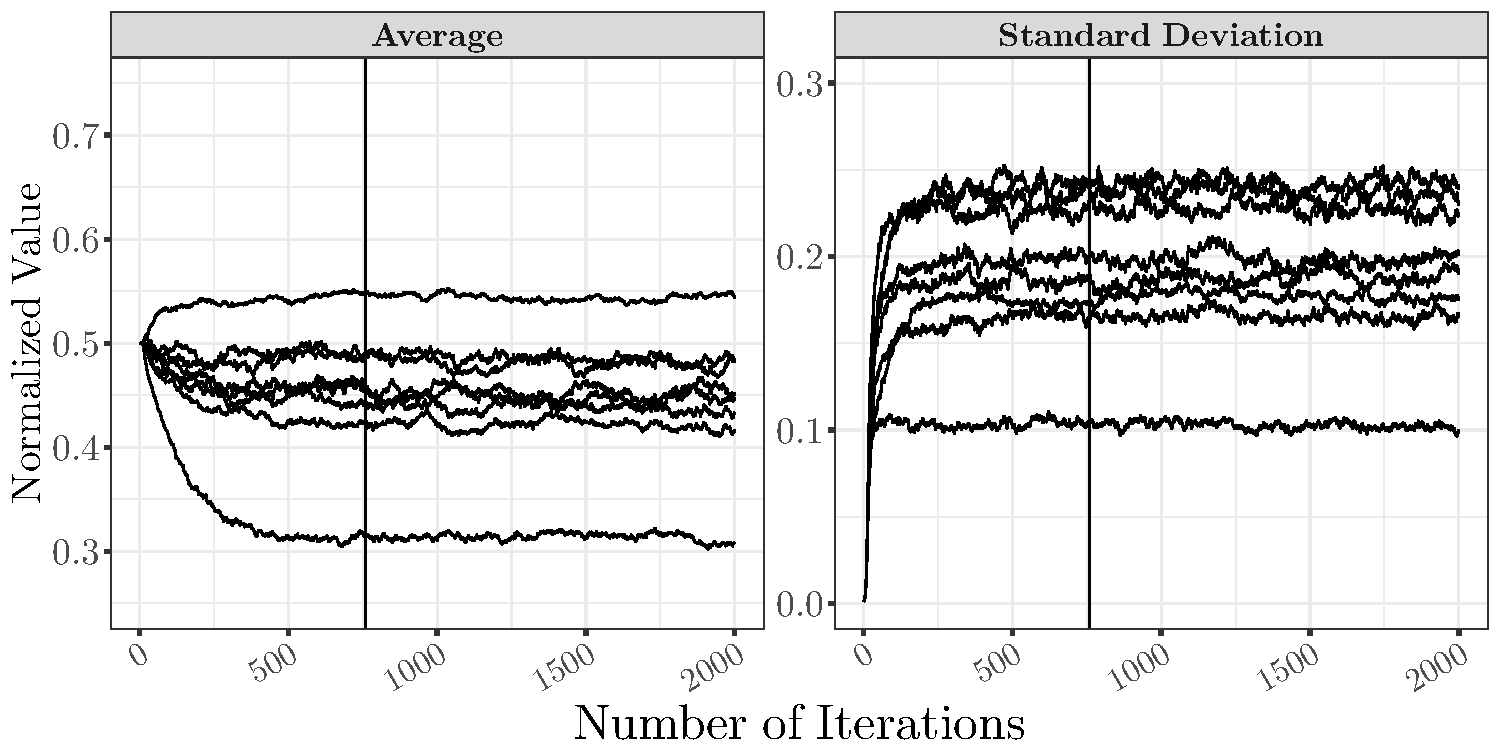
\includegraphics[width=1.0\textwidth]{../figures/chapter5/figures/plotEnsStatMCMC}
    \caption[Ensemble average and standard deviation as function of the number of iterations for calibration with model bias term.]{Ensemble average and standard deviation as function of the number of iterations for calibration with model bias term. Vertical lines indicate the iterations for burn-in (i.e., approximately $10$ times the autocorrelation time).}
    \label{fig:ch5_plot_ens_stat_mcmc}
\end{figure}

% Table of autocorrelation times, burn-in
Although the length of the burn-in period can be inferred directly from the plots in Fig.~\ref{fig:ch5_plot_ens_stat_mcmc}, a slightly more precise criteria can be obtained via the autocorrelation time of the running statistics.
Table~\ref{tab:ch5_ens_stat_mcmc} summarizes the estimated autocorrelation time for the running statistics and for each of the model parameters.
As can be seen, the autocorrelation times of the average tend to be longer than the ones of standard deviation. 
The longest autocorrelation time of all the parameters (shown in the table in bold) becomes the basis for determining the length of burn-in period.
As recommended in \cite{Sokal1997} a multiple (e.g., $10$) of the autocorrelation time is deemed enough to remove the initialization bias of the \gls[hyper=false]{mcmc}.
The obtained length of the burn-in period is shown as vertical lines in Fig.~\ref{fig:ch5_plot_ens_stat_mcmc} (at iteration $760$).
\begin{table}[h]
	\myfloatalign
	\caption[Estimated autocorrelation times for the $8$ model parameters with respect to the ensemble running average and standard deviation, for the calibration with model bias term.]{Estimated autocorrelation times for the $8$ model parameters with respect to the ensemble running average and standard deviation, for the calibration with model bias term. The bold term indicates the largest autocorrelation time used to determine the length of burn-in.}
	\label{tab:ch5_ens_stat_mcmc}
	\begin{tabularx}{1.05\textwidth}{rlccccc} \toprule
		\multirow{2}{*}{No.}&\multirow{2}{*}{Parameter}		&\multicolumn{2}{c}{Average}	&\phantom{a}&\multicolumn{2}{c}{Standard Deviation}\\
																												\cmidrule{3-4}	                           \cmidrule{6-7}
      &												& $\tau_{\text{pre-burn-in}}$ 	& $\tau_{\text{post-burn-in}}$	&& $\tau_{\text{pre-burn-in}}$ & $\tau_{\text{post-burn-in}}$ \\ \midrule
		\footnotesize{1}	&	\footnotesize{\texttt{gridHT}	}			  & \footnotesize{$64.3$}  				& \footnotesize{$6.8$} 	        && \footnotesize{$30.1$}  		 & \footnotesize{$26.6$}\\
		\footnotesize{2}	&	\footnotesize{\texttt{iafbWHT}} 			& \footnotesize{$31.6$} 				& \footnotesize{$22.5$} 	      && \footnotesize{$24.3$}  		 & \footnotesize{$21.8$}\\
		\footnotesize{3}	&	\footnotesize{\texttt{dffbWHT}} 			& \footnotesize{$51.1$}  				& \footnotesize{$29.9$} 	      && \footnotesize{$16.7$}  		 & \footnotesize{$16.8$}\\
		\footnotesize{4}	&	\footnotesize{\texttt{dffVIHT}}			  & \footnotesize{$66.3$}  				& \footnotesize{$22.3$} 	      && \footnotesize{$28.2$}  		 & \footnotesize{$14.4$}\\
		\footnotesize{5}	&	\footnotesize{\texttt{iafbIntDr}} 		& \footnotesize{$57.6$}  				& \footnotesize{$38.8$} 	      && \footnotesize{$21.8$}  		 & \footnotesize{$15.9$}\\
		\footnotesize{6}	&	\footnotesize{\texttt{dffbIntDr}} 		& \footnotesize{$\bm{75.5}$}  	& \footnotesize{$17.5$} 	      && \footnotesize{$18.5$}  		 & \footnotesize{$22.7$}\\
		\footnotesize{7}	&	\footnotesize{\texttt{dffbWDr}}			  & \footnotesize{$27.1$}  				& \footnotesize{$18.7$} 	      && \footnotesize{$50.1$}  		 & \footnotesize{$6.5$}\\
		\footnotesize{8}	&	\footnotesize{\texttt{tQuench}} 			& \footnotesize{$53.4$}  				& \footnotesize{$13.1$} 	      && \footnotesize{$28.2$}  		 & \footnotesize{$16.0$}\\
		\bottomrule
	\end{tabularx}
\end{table}

% Thinning
After such period, the decision on when to stop the \gls[hyper=false]{mcmc} simulation is the statistical precision of the parameters estimates.
The statistical precision is proportional to the square root of independent sample size.
Additionally, \gls[hyper=false]{mc} simulation for forward uncertainty quantification requires independent (specifically, iid) samples.
Therefore, to obtain the total number of independent samples, the remaining correlated samples are thinned on the basis of the autocorrelation time after burn-in.
As such, the auto-correlation times are recomputed after burn-in and given in Table~\ref{tab:ch5_ens_stat_mcmc}.
In the case of the calibration with model bias term, using the largest autocorrelation time ($\approx 39$) for thinning, $32'000$ posterior samples out of $1'240'000$ post-burn-in samples are independent and can be readily used for forward uncertainty propagation.
Though results in a much smaller sample size, the associated relative statistical error of the mean is at most $0.8\%$.